% Pruebas

Este capítulo tiene como objetivo presentar un plan de prueba(s) que permita corroborar los resultados obtenidos en el capitulo \ref{capres}. Este plan de pruebas esta diseñado para ser verificado mediante el sistema prototipo creado en este trabajo de grado y bajo las condiciones iniciales y otras consideraciones que se describen en este capítulo.

\section{Condiciones iniciales.}
Para corroborar el funcionamiento del sistema prototipo es necesario tener en cuenta algunas consideraciones, limitantes o condiciones iniciales tales como:

\begin{enumerate}
    \item De acuerdo con la emergencia sanitaria declarada por la Resolución 385 de marzo 12 de 2020, así como también el Decreto número 1-0666 del 12 de marzo de 2020 para el Valle del Cauca, se realizan las pruebas en el lugar de residencia y no en instalaciones externas como el campus de la universidad o alguno de sus laboratorios.
    \item Con base en el primer item, los circuitos o elementos de hardware se conectan en protoboard y no en circuito impreso.
    \item No se utilizan bovinos ni otros animales para el testeo del sistema prototipo.
    \item La implementación del mecanismo de la biela-manivela no es viable en las circunstancias actuales ocasionadas principalmente por la pandemia del COVID-19 y secundariamente a las dificultades descritas en la sección \ref{biela}.
    \item El alimento dietario utilizado para estas pruebas son lentejas ya que se aproximan en gran medida a la composición semi granulada y poco elástica del alimento utilizado en la ganadería.
    \item Los objetos o elementos utilizados para realizar, fabricar y/o evidenciar el funcionamiento de las partes del sistema son propiedad privada y en ninguna medida son propiedad de la Universidad.
    \item Los valores de los pesos dietarios son valores de prueba y no están proporcionalmente relacionados a los pesos que se obtengan en la etapa de pesaje. Esto quiere decir que no necesariamente existe la proporcionalidad o escalabilidad de una dieta teórica tal y como se describe en el Capítulo \ref{cap3}.
    \item Los eventos, nombres, partes o elementos nombrados que se mencionan en este trabajo de grado son ficticios o hipotéticos; cualquier similitud con la realidad es pura coincidencia.
\end{enumerate}

% \section{Funcionamiento}
A continuación se hace mención de los planes de prueba usados para corroborar el funcionamiento apropiado del sistema prototipo en cada una de sus etapas y en cada uno de los casos de análisis abarcados.

\section{Identificación de bovinos}
Para verificar la identificación de los bovinos se utiliza un lector RFID RC522  y accesorios RFID como los de la Figura \ref{rfidtagpng}. Una vez realizadas las conexiones y ejecutando el programa correspondiente, se debe acercar el accesorio RFID al lector.

\subsection{Caso 1: Identificación de novillo registrado}

 Si la referencia electrónica del accesorio se encuentra previamente registrada y asociada a un nombre de un bovino, la identificación de ese ``tag'' es exitosa  ocasionando que se ilumine un LED de color azul como indicador visual (ver figura \ref{idokpng}). 
 \begin{figure}[H]
    \centering
    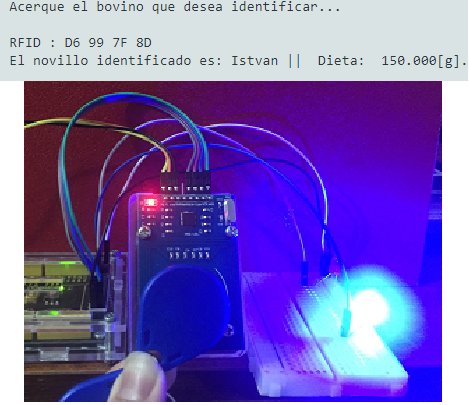
\includegraphics[scale=0.8]{img/idok.png}
    \caption{Caso 1: Identificación de novillo registrado.}
    \label{idokpng}
 \end{figure}
 
 \subsubsection{Caso 1.2: ``Novillo ya servido''} \label{idya}

En caso que el novillo identificado ya haya sido servido (\texttt{Served[j]=1}), se acciona una alarma sonora mediante un buzzer y una indicación visual al encender un LED de color rojo.

\subsection{Caso 2: Identificación de novillo no registrado}\label{idnpi}

 En caso de no ser identificado, el novillo es denominado como novillo no identificado, lo que acciona una alarma sonora mediante un buzzer y una indicación visual al encender un LED de color rojo (ver  figura \ref{idok2png}).
 
 \begin{figure}[H]
    \centering
    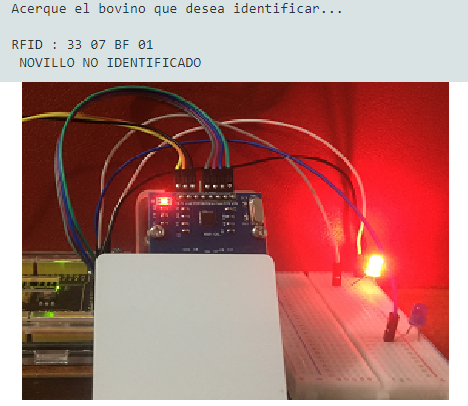
\includegraphics[scale=0.65]{img/idok2.png}
    \caption{Caso 2: Identificación de novillo no registrado.}
    \label{idok2png}
 \end{figure}
 

\section{Extracción del alimento}

Para lograr la extracción del alimento es necesario que se realicen las conexiones indicadas en la Tabla \ref{conexfood}. Una vez el programa haya sido ejecutado, es prerrequisito que el bovino haya sido identificado de manera exitosa. 
Se denomina una extracción exitosa si el tornillo se detiene cuando la gramera digital ofrece un valor igual o superior al valor de la dieta asociada al novillo identificado (ver ejemplo en la Figura \ref{extractokpng}).

\begin{figure}[H]
    \centering
    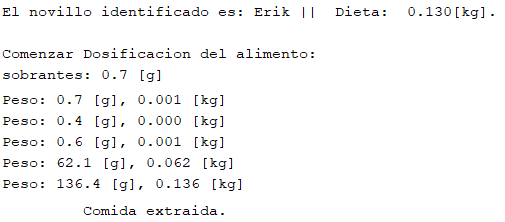
\includegraphics[scale=0.70]{img/extractok.png}
    \caption{Extracción exitosa del alimento.}
    \label{extractokpng}
\end{figure}

\section{Servir y detectar alimento en el plato}

Una vez que el alimento haya sido extraído de manera satisfactoria, el alimento debe ser servido dentro del plato. 
En situaciones ideales donde se cuente con la implementación del mecanismo de Biela-Manivela, el alimento es servido satisfactoriamente si:
\begin{enumerate}
    \item El valor que indica la gramera digital es nuevamente aproximadamente igual a cero o a un valor denominado como sobrante.
    \item Se denomina sobrante a partículas o restos de alimento o polvo situados en la superficie de la gramera digital al momento de realizar el pesaje.
    \item Alguno de los sensores infrarrojos indica detección de alimento independientemente del nivel que éste represente, es decir que su estado es igual a \texttt{1}.
    \item Tanto el ítem 1 como el ítem 3 deben cumplirse para detener el accionamiento del motor actuador del mecanismo de la biela-manivela
\end{enumerate}

En las circunstancias actuales a diferencia de una situación ideal, el cumplimiento de los ítems anteriores simplemente no accionará al motor actuador. Esto puede verificarse mediante el monitor serial tal y como se muestra en la Figura \ref{servedokpng}.

\begin{figure}[H]
    \centering
    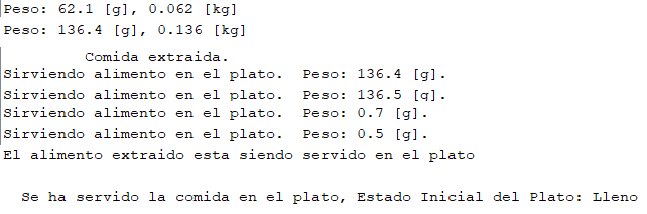
\includegraphics[scale=0.7]{img/servedok.png}
    \caption{Alimento satisfactoriamente servido en el plato.}
    \label{servedokpng}
\end{figure}

% \section{Temporizador}
% El funcionamiento del temporizador puede corroborase al 
\section{Estado del plato}

El estado del plato podrá tener los siguientes valores:
\begin{enumerate}
    \item Lleno: El plato se encuentra ``lleno'' si el sensor infrarrojo más alto detecta alimento, esto se puede observar cuando el sensor infrarrojo ilumine un LED de color rojo.
    \item Medio: El plato se encuentra ``medio'' si el sensor infrarrojo de la mitad detecta alimento, esto se puede observar cuando el sensor infrarrojo ilumine un LED de color rojo.
    \item Bajo: El plato se encuentra ``bajo'' si el sensor infrarrojo más bajo detecta alimento, esto se puede observar cuando el sensor infrarrojo ilumine un LED de color azul.
    \item Vacío: El plato se encuentra ``vacío'' si ningún sensor infrarrojo detecta alimento.
\end{enumerate}

\section{Pesaje del bovino}

\begin{enumerate}
    \item Para pesar a un bovino es necesario que el temporizador y la etapa de consumo de alimento hayan finalizado.
    \item Debe procederse a posicionar al bovino encima de la superficie de la báscula de pesado.
    \item Una vez el peso detectado por la báscula converja a un valor estable o poco variable, se debe presionar y mantener presionado durante unos 2 segundos el botón que permite almacenar ese valor y detener la medición en la báscula (ver Figura \ref{pesookpng}).
    \begin{figure}[H]
        \centering
        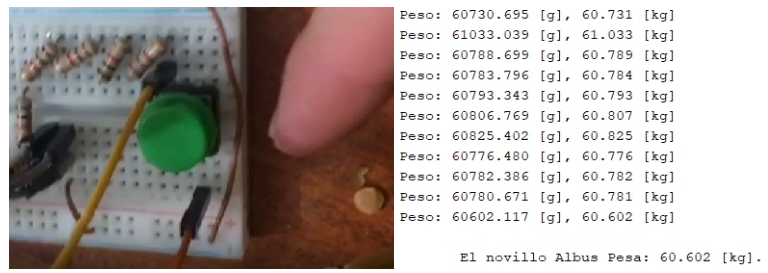
\includegraphics[scale=0.7]{img/pesook.png}
        \caption{Almacenamiento de peso por pulsación de botón.}
        \label{pesookpng}
    \end{figure}
\end{enumerate}
  
\section{Alarmas}

\subsection{ID erróneo}
Ver sección \ref{idnpi}.

\subsection{ID repetido}
Ver sección \ref{idya}.

\subsection{Alimento no consumido}

Se registra la activación de una alarma por alimento no consumido cuando el estado final del plato sea diferente al estado ``Vacio'' (ver Figura \ref{eatenalpng}). Esto sin importar que se haya consumido parte del alimento (transiciones de ``Lleno'' a ``Medio'', ``Lleno'' a ``Bajo'' o ``Medio'' a ``Bajo'').
Esta alarma también es accionada si el estado inicial del plato coincide con el estado final considerando a este como una situación en la que no se consumió alimento.

\begin{figure}[H]
    \centering
    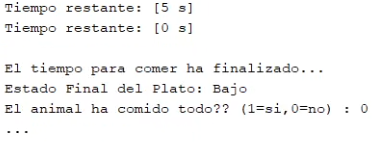
\includegraphics[scale=1.25]{img/eatenal.png}
    \caption{Registro de alarma por motivo de alimento no consumido.}
    \label{eatenalpng}
\end{figure}

\subsection{Alimento insuficiente en el tanque}

Se registra la activación de una alarma por alimento insuficiente en el tanque cuando el valor de alimento existente en éste sea menor al valor mínimo requerido para dar abasto a un posible próximo ejemplar que represente al ``peor de los casos'' tal y como se menciona en la sección \ref{lvltolva} ($Vmin=480[g]$).\\

Es importante aclarar que esta alarma es un indicador que sirve como referencia a que el alimento almacenado en el tanque esta próximo a acabarse, mas sin embargo el sistema puede operar para aquellos ejemplares cuyo valor dietario sea menor a ese valor mínimo requerido (ver Figura \ref{tankalpng}).

\begin{figure}[H]
    \centering
    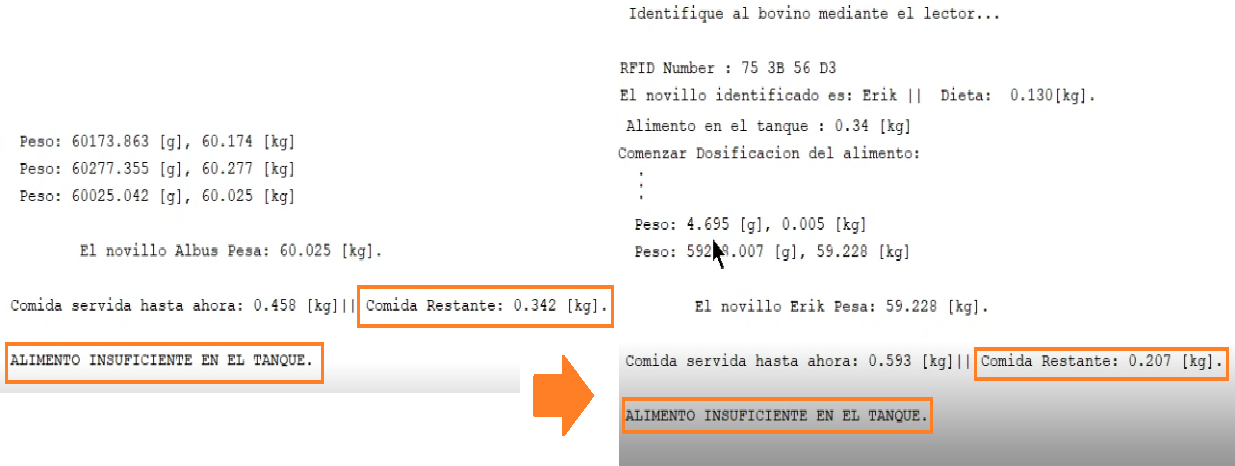
\includegraphics[scale=0.5]{img/tankal.png}
    \caption{Registro de alarma por motivo de alimento insuficiente en el tanque.}
    \label{tankalpng}
\end{figure}
\pagebreak

\section{Registro de datos}

\begin{enumerate}
    \item El registro de los datos se realiza en un archivo de texto con extensión \textt{.txt}.
    \item Este archivo poseerá renglones de texto con 14 o 15 columnas diferentes (dependiendo si se considera la columna de iteración).
    \item Cada columna representa a los datos de interés descritos en el Capítulo \ref{capres}, en la sección \ref{datosinteres}.
    \item Si no hay datos que registrar el campo existente entre dos ``punto y coma (\textt{;})'' será nulo (\textt{\ldots;;\ldots}).
\end{enumerate}

\subsection{Caso 1: Identificación exitosa}

Suponiendo que la identificación del ejemplar \textt{n}-ésimo fue exitosa, los datos de interés mencionados en la sección \ref{datosinteres} son debidamente almacenados en variables que ayudan a describir la situación de la iteración \textt{n}-ésima.

Una vez finalizada esta iteración de adquisición de datos correspondiente al bovino \textt{n}-ésimo se reescribe el archivo de texto ubicado en la memoria micro SD con un nuevo renglón de datos separados por un ``punto y coma'' (ver iteraciones 1, 3 o 5 en la Figura \ref{ejsdtxtpng}).\\

Nótese que en este caso, se obtendrá un total de 15 columnas compuestas por 1 columna que indica la iteración \textt{n}-ésima y otras 14 columnas con los datos que se hayan adquirido. 

\subsection{Caso 2: Identificación no exitosa}

Suponiendo que la identificación del ejemplar \textt{n}-ésimo no fue exitosa, la única columna del renglón registrado en el archivo de texto de la memoria micro SD que tendrá un valor no nulo, es la columna \#4 que hace referencia a la activación de una alarma por motivo de un novillo no identificado (ver iteración 2 en la Figura \ref{ejsdtxtpng}).

\subsection{Caso 3: Identificación repetida de bovino}

Suponiendo que la identificación del ejemplar \textt{n}-ésimo fue exitosa y además es un bovino previamente identificado, sólo se tendrán valores no nulos en las primeras 5 columnas (incluyendo la columna de iteración). Las columnas siguientes tendrán un valor nulo dado que no se adquieren datos para bovino pre identificados (Ver iteración 4 en la Figura \ref{ejsdtxtpng}).\\
\pagebreak

\begin{figure}[H]
    \centering
    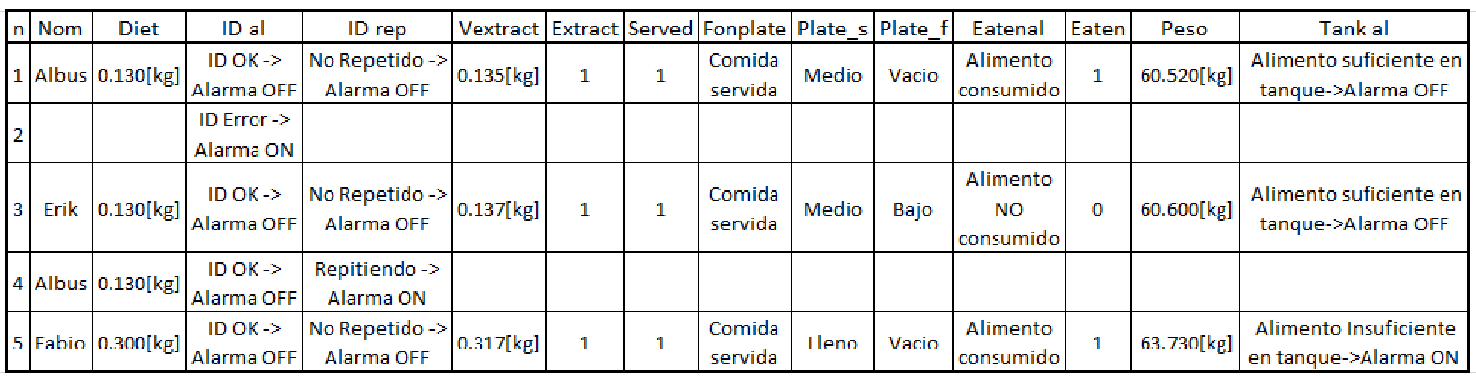
\includegraphics[scale=0.5, angle=90]{img/ejsdtxt.png}
    \caption{Registro de renglón de datos separados por ``punto y comas''.}
    \label{ejsdtxtpng}
\end{figure}
